
\documentclass[border=50pt, tikz]{standalone}

% Circuits
\usepackage[european,s traightvoltages, RPvoltages, americanresistor, americaninductors]{circuitikz}
\tikzset{every picture/.style={line width=0.2mm}}

% Tikz Library
\usetikzlibrary{calc}

% Bipoles Specifications
\ctikzset{bipoles/thickness=1.2, label distance=1mm, voltage shift = 1}

\def\nu{10}
\definecolor{myblue}{HTML}{ABDCEC}

\begin{document}
	
	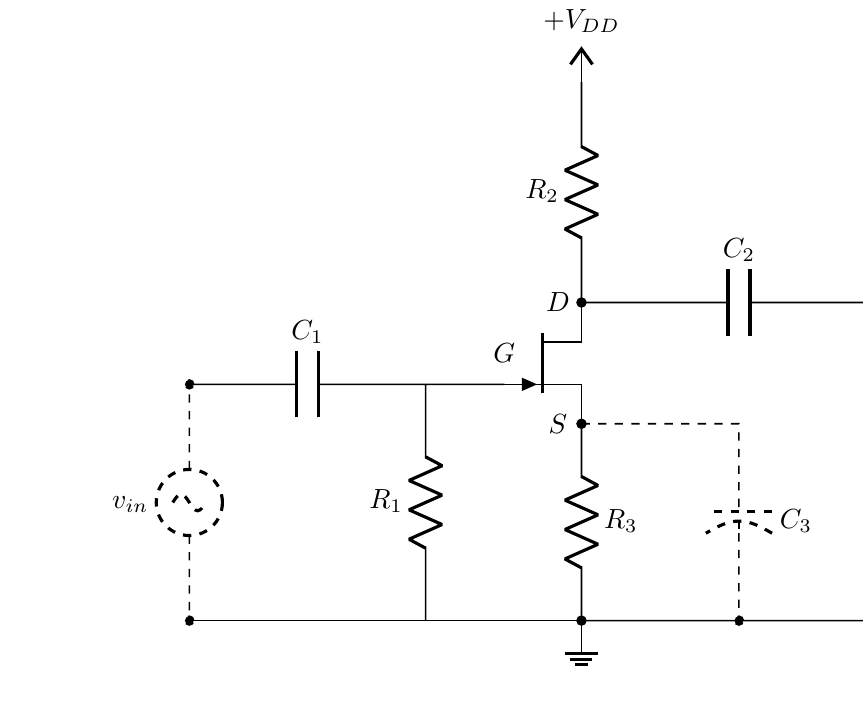
\begin{tikzpicture}
	\begin{circuitikz}
		\ctikzset{voltage/american plus/.initial={}, voltage/american minus/.initial={}}
	
%		%Grid
%		\draw[thin, dotted] (0,0) grid (\nu,\nu);
%		\foreach \i in {1,...,\nu}
%		{
%			\node at (\i,-2ex) {\i};	
%		}
%		\foreach \i in {1,...,\nu}
%		{
%			\node at (-2ex,\i) {\i};	
%		}
%		\node at (-2ex,-2ex) {0};
		
		%Coordinates
		\node[njfet] (Q) at (5,3.5) {};
		
		% Circuit
		\draw
		
		(Q.S) node[shift={(-0.3,0)}] {$S$} to[R, l^=$R_3$, *-*] ++(0,-2.5) node[ground] (GR) {}
		
		(Q.D) node[shift={(-0.3,0)}] {$D$} to[R, l^=$R_2$, *-] ++(0,2.8) node[vcc] {$+V_{DD}$}
		(Q.D) to[C, l^=$C_2$] ++(4,0) -- ++(0,-1.35) node (D') {} 
			  to[open, v=$v_o$, o-o, american] ++(0,-1.3) -- (GR -| D') -- (GR)
		
		(Q.G) node[shift={(0,0.4)}] {$G$} -- ++(-1,0) node[inner sep=0, outer sep=-1] (G') {} to[R, l_=$R_1$] (GR -| G')
		(G') to[C, l_=$C_1$] ++(-3,0) node (G'') {};
		
		\draw (GR) -- (GR -| G'');
		
		\draw[dashed]
		(Q.S) -- ++(2,0) to[curved capacitor, l^=$C_3$, -*] ++(0,-2.5)
		(G'') to[sV, l_=$v_{in}$, *-*] (G'' |- GR);
		
	\end{circuitikz}
	\end{tikzpicture}
	
	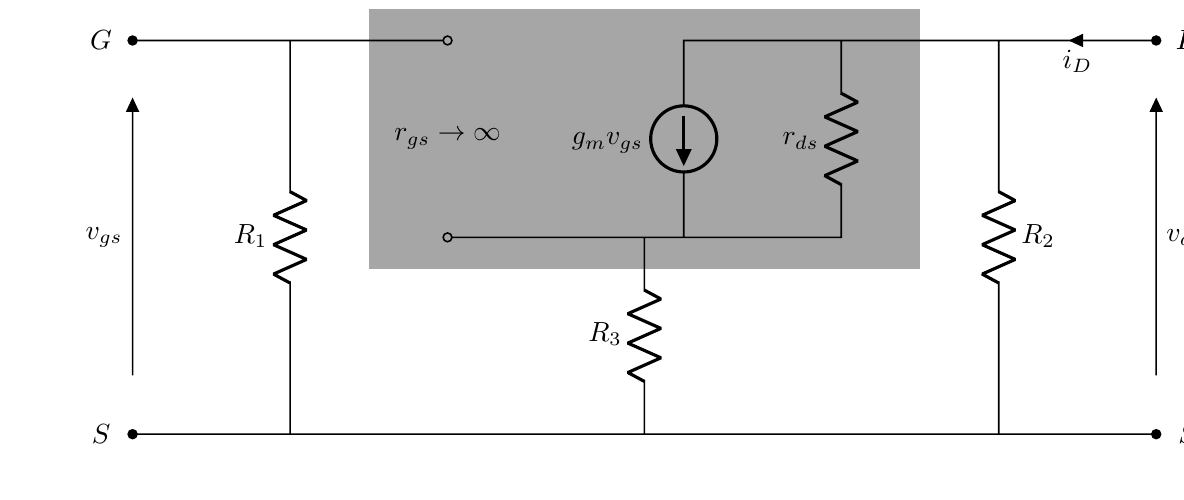
\begin{tikzpicture}
	\begin{circuitikz}
		\ctikzset{voltage/american plus/.initial={}, voltage/american minus/.initial={}}
	
%		% Grid
%		\draw[thin, dotted] (0,0) grid (\nu,\nu);
%		\foreach \i in {1,...,\nu}
%		{
%			\node at (\i,-2ex) {\i};	
%		}
%		\foreach \i in {1,...,\nu}
%		{
%			\node at (-2ex,\i) {\i};	
%		}
%		\node at (-2ex,-2ex) {0};

		% Coordinates		
		\coordinate (G) at (0,5);
		\coordinate (S) at (0,0);
		
		% Circuit
		\draw
		
		% Left Part					
		(G) node[shift={(-0.4,0)}] {$G$} to [open, v_=$v_{gs}$, *-*] (S) node[shift={(-0.4, 0)}] {$S$}
		(G) -- ++(4,0) coordinate (G) to [open, v=$r_{gs}\to\infty$, o-o, american] ++(0,-2.5) coordinate (ML)
		
		(S) -- ++(2,0) coordinate (SL) to [R, l^=$R_1$] (SL |- G) coordinate (G')
		
		(SL) -- ++(2,0)
		
		% Right Part
		(ML) -- ++ (3,0) coordinate (MR) to [american current source, l^=$g_mv_{gs}$, invert] ++(0,2.5)
			  -- ++(6,0) coordinate (D) node[shift={(0.4, 0)}] {$D$}
			  
		(MR) -- ++(2,0) coordinate (MR') to [R, l^=$r_{ds}$] (MR' |- D) coordinate (D'')
		
		($(ML)!0.5!(MR')$) to [R, l_=$R_3$] ++(0,-2.5) coordinate (SM) -- (S)
		
		(D'') -- ++(2,0) coordinate (D') to [R, l^=$R_2$] (D' |- S) coordinate (SR')
		
		(SR') -- (SR' -| D) coordinate (SR)
		(SR') -- (SM)
		
		(D) node[shift={(0.4,0)}] {$D$} to [open, v^=$v_{ds}$, *-*] (SR) node[shift={(0.4, 0)}] {$S$}
		(D) to [short, i=$i_{D}$] (D');
		
		% Rectangle
		\draw[draw=none, fill=black, fill opacity=0.35] ($(ML) - (1,0.4)$) rectangle ($(D'')!0.5!(D') + (0,0.4)$);
		
	\end{circuitikz}
	\end{tikzpicture}
	
\end{document}
